\begin{scanpage}{0109}{92}
\noindent\begin{minipage}[t]{.48\linewidth}\vspace{0pt}\centering
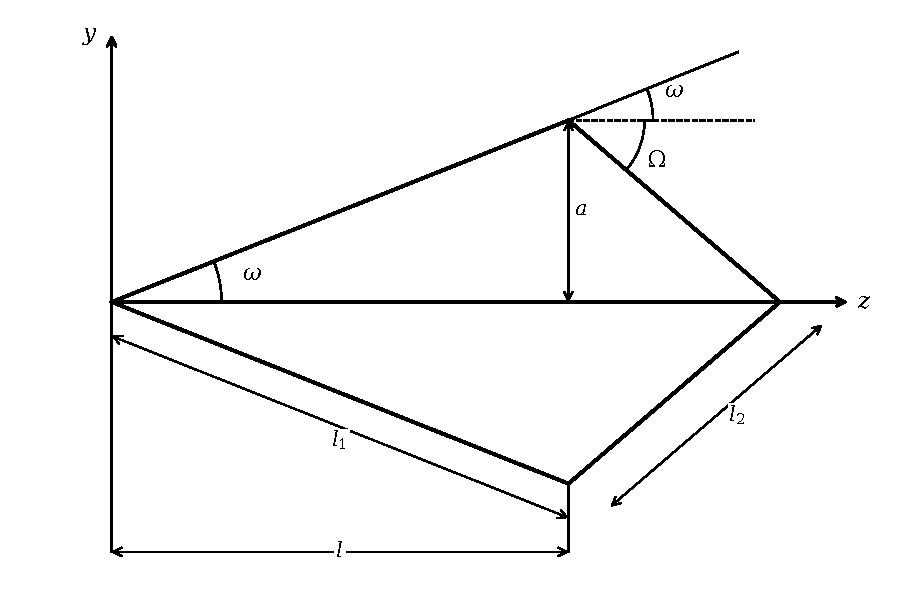
\includegraphics[width=.9\linewidth]{images/recreated/b-0109-fig28.pdf}

Figure 28. Diffraction of a plane wave by a conical body. The plane wave is propagated along the $z$ axis.
\end{minipage}\hfill\begin{minipage}[t]{.48\linewidth}\vspace{0pt}\centering
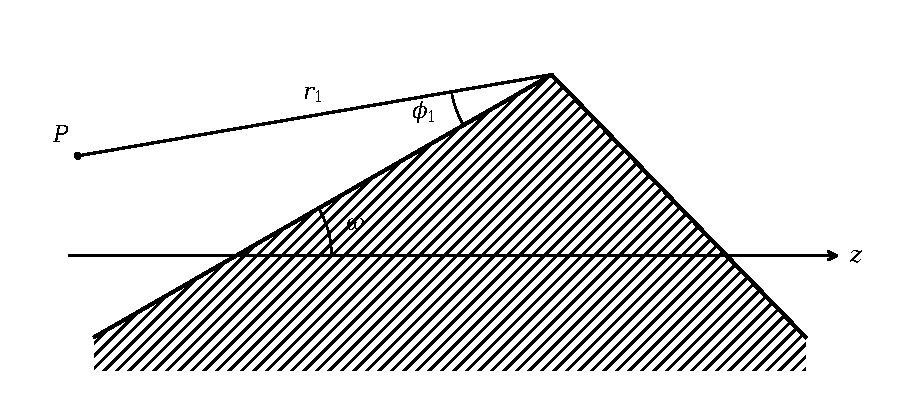
\includegraphics[width=.95\linewidth]{images/recreated/b-0109-fig29.pdf}

Figure 29. The dihedral angle corresponding to the discontinuity of a conical surface.

\raggedright of the current flowing on such a wedge is determined in the
\end{minipage}\par\medskip

far zone $(kr_1\gg1)$ by the following equations:
\[\left.\begin{aligned}E_{z_1}(\psi)&=-H_{\phi_1}(\psi)=ikA_{z_1}(\psi),\\H_{z_1}(\psi)&=E_{\phi_1}(\psi)=ikA_{\phi_1}(\psi),\end{aligned}\right\}\tag{16.06}\]
where
\[\begin{aligned}\mathbf A={}&\frac1c\sqrt{\frac{2\pi}{k_1r_1}}\left[\int_0^\infty\mathbf j_1^1(\zeta)e^{\pm ik\zeta\cos\omega}d\zeta\right.\\&\left.\quad+\int_0^\infty\mathbf j_2^1(\zeta)e^{\mp ik\zeta\cos\Omega}d\zeta\right]e^{i(kr_1+\pi/4)}.\end{aligned}\tag{16.07}\]
Here the upper sign in the exponents refers to the case $\phi_1=\pi+\omega$, and the lower sign --- to the case $\phi_1=\omega$. On the other hand, in \S\ 4 it was shown that this field equals
\[\left.\begin{aligned}E_{z_1}(\psi)&=E_{0z_1}(\psi)f^1\frac{e^{i(kr_1+\pi/4)}}{\sqrt{2\pi kr_1}},\\H_{z_1}(\psi)&=H_{0z_1}(\psi)g^1\frac{e^{i(kr_1+\pi/4)}}{\sqrt{2\pi kr_1}},\end{aligned}\right\}\tag{16.08}\]
where $E_{0z_1}(\psi)$, $H_{0z_1}(\psi)$ are the values of the incident wave amplitude at the wedge edge, and $f^1$ and $g^1$ are angular functions characterizing the scattering diagram.
\end{scanpage}
